\section{Reweight of Different Hadronic Tau Decay Modes in the Simulation}
\label{sec:app:tauBr}

The MC events with $\tau_h$ in the $e\tau$ and $\mu \tau$ channel is essential to the sensitivity of the
$Br(W\to\tau)$ measurement. However, the tau's hadronic decay branching fraction $B(\tau \to  \rm{hadrons})$
in the MC simulation are different from the experimental world average in the PDG.
The $\tau_h$ selection efficiency could be impacted by such difference because various tau's hadronic 
decay mode have different efficiencies in the CMS $\tau_h$ reconstruction with SPH algorithm.

Thus it is necessary to reweight the MC events to correct the deviation of tau's decay in the simulation
with respect to the PDG values. For the values in the \PYTHIA simulation assumption and the PDG world average,
tau's hadronic decay branching fractions are listed in table~\ref{tab:tauhReweighting}. The difference between 
values in \PYTHIA8 and PDG is about $0.5\%$. The ratios of PDG and
\PYTHIA values are also included, which are the event weights applied for the $\tau \to h$ reweighting.

    
    
\begin{table}[ht]
  \centering
  \setlength{\tabcolsep}{1 em}
  \renewcommand{\arraystretch}{1.5}
  \caption{ The values of $B(\tau \to  \rm{hadrons})$ in PYTHIA8 and in PDG.}
  \begin{tabular}{l|c|c|c}
  \hline
                              & PDG        & \PYTHIA   & PDG / \PYTHIA \\
  \hline
  $B(\tau\to \pi^\pm)$       & 0.1082(5)  & 0.1076825 & 1.00481       \\
  $B(\tau\to \pi^\pm+ \pi^0)$& 0.2549(9)  & 0.2537447 & 1.00455       \\
  $B(\tau\to \pi^\pm+2\pi^0)$& 0.0926(10) & 0.0924697 & 1.00141       \\
  $B(\tau\to3\pi^\pm)$       & 0.0931(5)  & 0.0925691 & 1.00574       \\
  $B(\tau\to3\pi^\pm+ \pi^0)$& 0.0462(5)  & 0.0459365 & 1.00574       \\
  \hline
  \end{tabular}
  \label{tab:tauhReweighting}
\end{table}


\begin{figure}
    \centering
    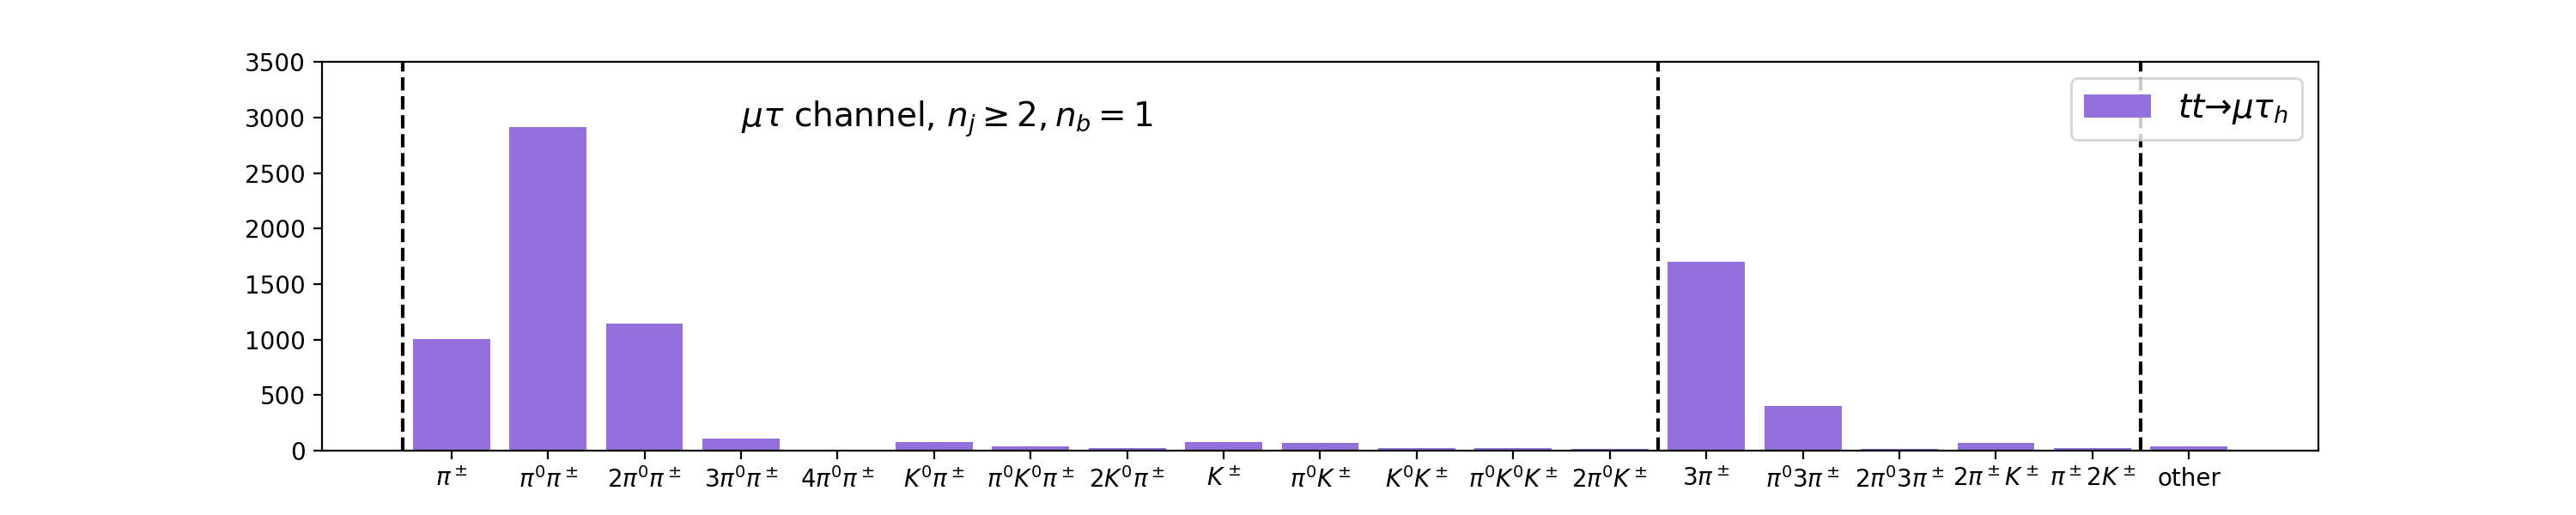
\includegraphics[width=0.99\textwidth]{chapters/Appendix/sectionTauBr/figures/tauhDecay_mutau.png}
    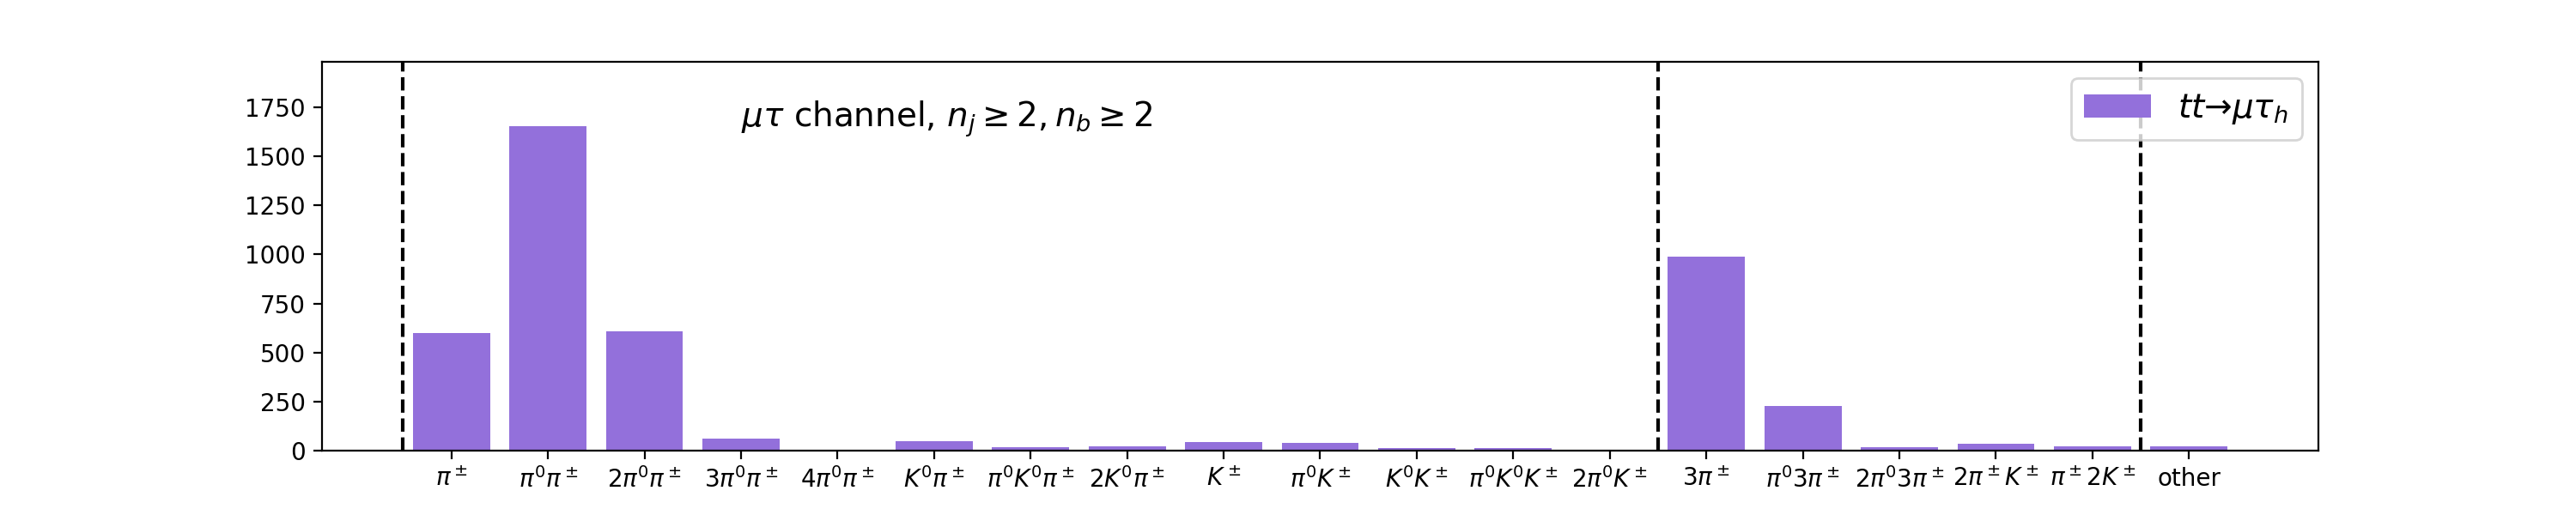
\includegraphics[width=0.99\textwidth]{chapters/Appendix/sectionTauBr/figures/tauhDecay_mutau2.png}
    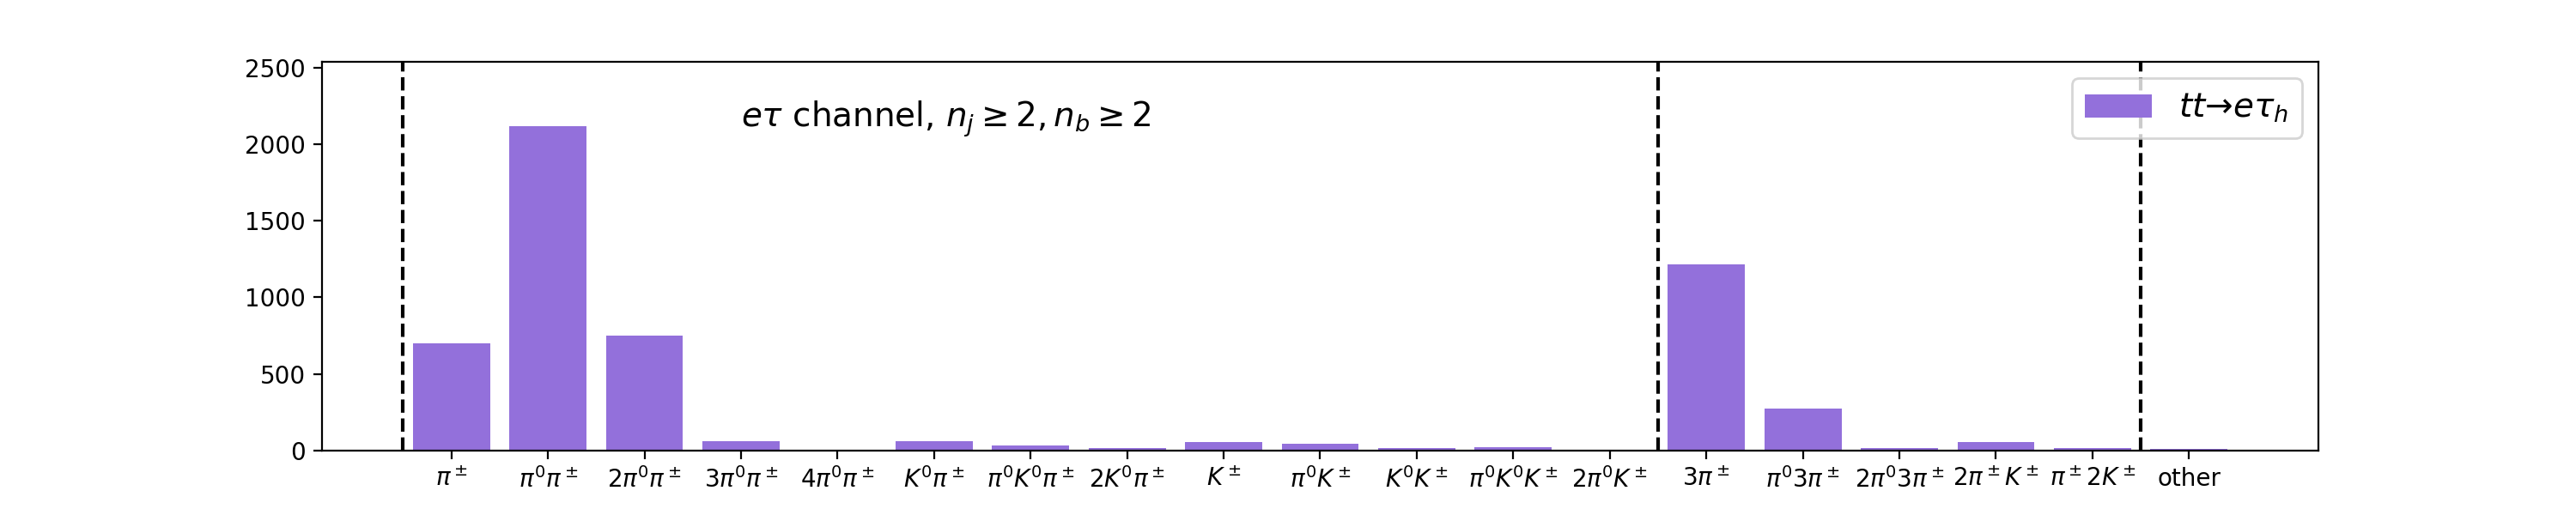
\includegraphics[width=0.99\textwidth]{chapters/Appendix/sectionTauBr/figures/tauhDecay_etau.png}
    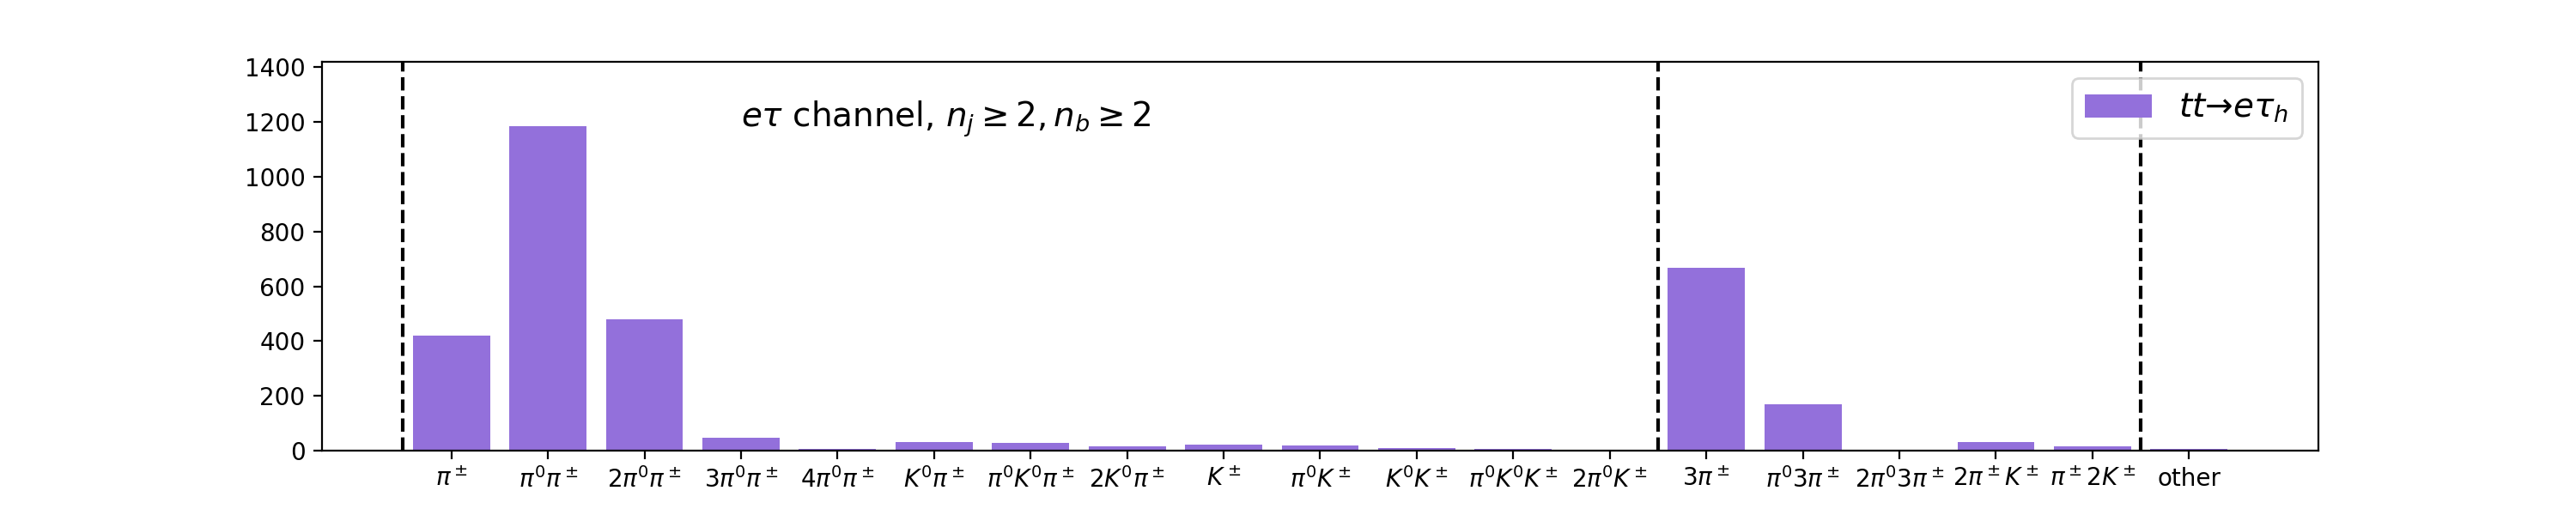
\includegraphics[width=0.99\textwidth]{chapters/Appendix/sectionTauBr/figures/tauhDecay_etau2.png}
    \caption{The gen-level daughter mesons from hadronicly decaying taus in the $tt\to \mu \tau_h, e \tau_h$ events passing $\mu \tau$ and $e \tau$ selection.}
    \label{fig:appendix:reweightTauhBr:tauhBr}
\end{figure}


In MC events, the gen-level daughter mesons from hadronically decaying taus are saved. 
The $\tau_h$'s daughter mesons in the $tt\to \mu \tau_h, e \tau_h$ events 
passing $\mu \tau$ and $e \tau$ selection are shown
in Fig~\ref{fig:appendix:reweightTauhBr:tauhBr}
The leading contributions to the reconstructed $\tau_h$ are 
$\tau\to \pi^\pm+\pi^0 $, $\tau\to 3\pi^\pm$, $\tau\to \pi^\pm+2\pi^0$, $\tau\to
\pi^\pm$, $\tau\to 3\pi^\pm + \pi^0$. 
MC events with taus in those five decay modes are reweighted by 

\begin{equation}
  w = \frac{^{\rm PDG} B(\tau \to  \rm{hadrons}) }{^{\rm \PYTHIA} B( \tau \to \rm{hadrons} )}. 
\end{equation} 


\noindent The uncertainties of the weights are from the the PDG uncertainties. 
The systematical uncertainty due to the uncertainties of $B(\tau \to  \rm{hadrons})$ 
reweighting can be estimated. The effect of the $B(\tau \to  \rm{hadrons})$ 
reweighting on the $B(W)$ result is small. The relative
systematics from $B(\tau \to  \rm{hadrons})$ reweighting are about $0.003 - 0.146 \%$, 
shown in table~ \ref{tab:syst_tauhReweighting}.



\begin{table}[p]
  \centering
  \caption{ Relative systematic uncertainty ($\%$) due to $B(\tau \to  \rm{hadrons})$ reweighting.}
  \setlength{\tabcolsep}{0.5 em}
  \renewcommand{\arraystretch}{2}
  \resizebox{\textwidth}{!}{
  \begin{tabular}{|l|ccc|ccc|ccc|ccc|ccc|}
    \hline
    Error Source & \multicolumn{3}{c|}{$\mu$-1b} & \multicolumn{3}{c|}{$\mu$-2b} & \multicolumn{3}{c|}{$e$-1b} & \multicolumn{3}{c|}{$e$-2b} \\
    \hline
                  & $B_e$ & $B_\mu$ & $B_\tau$ & $B_e$ & $B_\mu$ & $B_\tau$ & $B_e$ & $B_\mu$ & $B_\tau$ & $B_e$ & $B_\mu$ & $B_\tau$ \\
    \hline
    0.5$\%$ err of $Br_{\tau\to\pi^\pm}$       & 0.009 & 0.013 & 0.055 & 0.009 & 0.012 & 0.051 & 0.009 & 0.012 & 0.052 & 0.010 & 0.012 & 0.057 \\ 
    0.5$\%$ err of $Br_{\tau\to\pi^\pm\pi^0}$  & 0.025 & 0.033 & 0.141 & 0.026 & 0.033 & 0.147 & 0.024 & 0.032 & 0.146 & 0.025 & 0.032 & 0.146 \\ 
    0.2$\%$ err of $Br_{\tau\to\pi^\pm2\pi^0}$ & 0.003 & 0.004 & 0.017 & 0.003 & 0.004 & 0.015 & 0.003 & 0.004 & 0.017 & 0.003 & 0.004 & 0.019 \\ 
    0.6$\%$ err of $Br_{\tau\to3\pi^\pm}$      & 0.017 & 0.022 & 0.101 & 0.019 & 0.023 & 0.111 & 0.017 & 0.023 & 0.107 & 0.017 & 0.022 & 0.107 \\ 
    0.6$\%$ err of $Br_{\tau\to3\pi^\pm\pi^0}$ & 0.005 & 0.006 & 0.024 & 0.005 & 0.006 & 0.022 & 0.004 & 0.006 & 0.022 & 0.005 & 0.006 & 0.025 \\ 
    \hline
  \end{tabular}}
  \label{tab:syst_tauhReweighting}
\end{table}
\FloatBarrier
